% =====================================================================
% ejercicio07.tex
% Responsabilidad única: ajustar la regresión múltiple estandarizada y la cuadrícula de árboles de
% regresión, y seleccionar con validación el candidato final de regresión.
% Las cifras provienen de generado/resultados.tex y generado/tabla_*.tex.
% =====================================================================
\subsection{Ejercicio 7 --- Caso A: regresión múltiple y árbol de regresión}

\begin{enumerate}

\item \textbf{Regresión múltiple con \texttt{Pipeline}.}
Se construyó un \texttt{Pipeline} con \texttt{StandardScaler} y
\texttt{LinearRegression}, de modo que medias y desviaciones se aprenden solo
con entrenamiento. El modelo múltiple obtuvo un RMSE de validación de
$\RegMultiRMSEVal$ (frente a $\RegSimpleRMSEVal$ del simple y
$\RegDummyRMSEVal$ de la constante) y un $R^2$ de validación de
$\RegMultiRdosVal$ (frente a $\RegSimpleRdosVal$), véase la
Tabla~\ref{tab:ex7-candidatos}. La mejora en entrenamiento (RMSE de
$\RegSimpleRMSETr$ a $\RegMultiRMSETr$) por sí sola no prueba nada, pues como
se justificó en el Ejercicio~2e añadir predictores nunca aumenta el error
mínimo de entrenamiento; lo relevante es que la mejora se conserva en
validación y que la brecha entre particiones no se abre.

\item \textbf{Coeficientes estandarizados y correlaciones.}
Cada coeficiente (Tabla~\ref{tab:ex7-coef}) es el cambio esperado en la
predicción ante un aumento de una desviación estándar de entrenamiento (la
poblacional que usa \texttt{StandardScaler}) en ese predictor, manteniendo
fijos los demás. Para \texttt{s5} un aumento de una desviación
($\DesvMultiScinco$ en el logaritmo de los triglicéridos) se asocia con
$\CoefMultiScinco$ unidades más de progresión, y para \texttt{bmi} un aumento
de una desviación ($\DesvMultiBmi$\,kg/m$^2$) se asocia con
$\CoefMultiBmi$ unidades más, equivalentes a unas $\BmiPorUnidad$ por
kg/m$^2$, cerca de la mitad de la pendiente simple ($\SimpleBetaUno$), ya que
allí \texttt{bmi} absorbía parte de lo que ahora explican predictores
correlacionados con él.

\begin{table}[H]
\centering
\small
% Archivo generado automáticamente por el notebook (no editar a mano).
\begin{tabular}{lrrr}
\toprule
Predictor & Coeficiente & Desv. est. (ent.) & Corr. con $y$ (ent.) \\
\midrule
s1 & $-$51.1014 & 35.2232 & 0.1623 \\
s5 & 37.2716 & 0.5015 & 0.5645 \\
s2 & 27.4808 & 31.2424 & 0.1073 \\
bmi & 25.0766 & 4.3741 & 0.5954 \\
bp & 15.1673 & 14.0075 & 0.4197 \\
s4 & 15.0321 & 1.2713 & 0.4076 \\
sex & $-$11.3593 & 0.4999 & $-$0.0275 \\
s3 & 10.8403 & 12.2802 & $-$0.3798 \\
s6 & 3.8171 & 11.4005 & 0.3867 \\
age & 1.1318 & 12.7451 & 0.2061 \\
\bottomrule
\end{tabular}

\caption{Coeficientes estandarizados de la regresión múltiple, ordenados por magnitud absoluta (entrenamiento).}
\label{tab:ex7-coef}
\end{table}

La matriz de correlaciones (Figura~\ref{fig:ex7-corr}) muestra pares
fuertemente relacionados, en especial \texttt{s1} y \texttt{s2}
($\CorrSunoSdos$) y \texttt{s3} y \texttt{s4} ($\CorrStresScuatro$). El caso
de \texttt{s1} y \texttt{s2} ilustra el problema, pues ambos tienen
correlación positiva con la variable objetivo ($\CorrYSuno$ y $\CorrYSdos$),
pero el modelo les asigna coeficientes de signo opuesto y gran magnitud
($\CoefMultiSuno$ y $\CoefMultiSdos$), porque al moverse casi juntos el
ajuste aprovecha su diferencia y no el nivel de cada uno; algo similar ocurre
con \texttt{s3}, de correlación negativa con el \emph{target}
($\CorrYStres$) y coeficiente positivo ($\CoefMultiStres$). Por esto los
coeficientes deben leerse como efectos parciales condicionados al resto,
inestables ante colinealidad, y no como importancias independientes.

\begin{figure}[H]
    \centering
    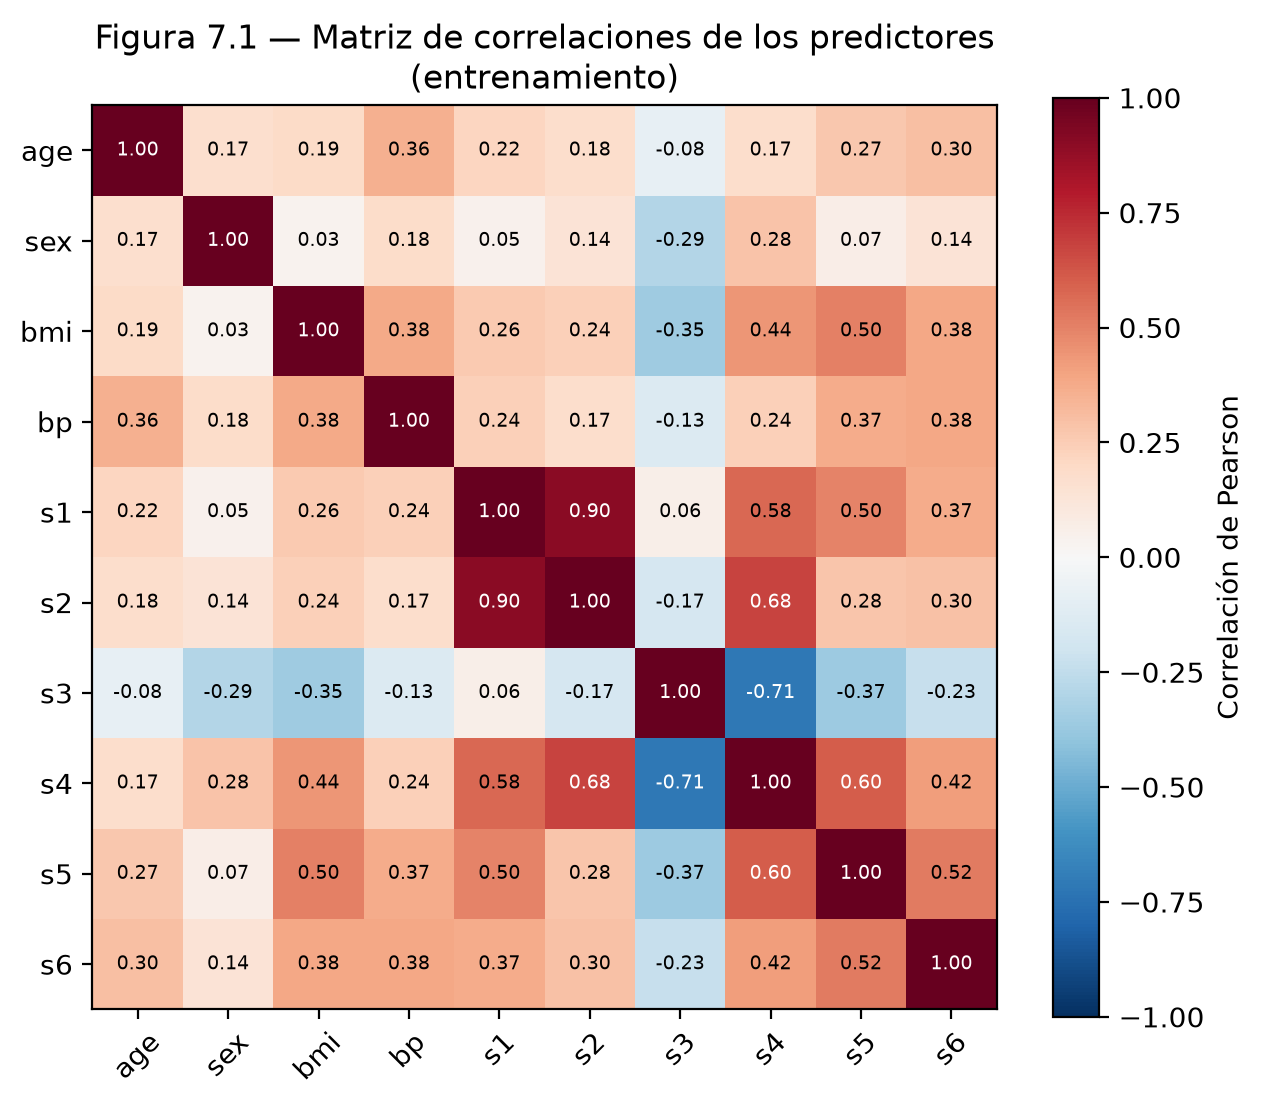
\includegraphics[width=0.62\textwidth]{figuras/ex7_correlaciones.png}
    \caption{Matriz de correlaciones de los predictores (entrenamiento).}
    \label{fig:ex7-corr}
\end{figure}

\item \textbf{Cuadrícula de \texttt{DecisionTreeRegressor}.}

\begin{table}[H]
\centering
\small
% Archivo generado automáticamente por el notebook (no editar a mano).
\begin{tabular}{rrrrrrr}
\toprule
max\_depth & min\_samples\_leaf & RMSE ent. & RMSE val. & Prof. real & Hojas & Brecha \\
\midrule
2 & 5 & 57.6273 & 58.7814 & 2 & 4 & 1.1541 \\
2 & 15 & 57.6273 & 58.7814 & 2 & 4 & 1.1541 \\
2 & 30 & 59.0808 & 57.3406 & 2 & 4 & $-$1.7402 \\
4 & 5 & 49.0068 & 61.0539 & 4 & 15 & 12.0471 \\
4 & 15 & 52.7463 & 58.1889 & 4 & 10 & 5.4425 \\
4 & 30 & 58.0732 & 56.7789 & 4 & 6 & $-$1.2943 \\
6 & 5 & 38.5411 & 63.2140 & 6 & 31 & 24.6729 \\
6 & 15 & 52.1941 & 57.9781 & 6 & 12 & 5.7840 \\
6 & 30 & 58.0732 & 56.7789 & 4 & 6 & $-$1.2943 \\
\bottomrule
\end{tabular}

\caption{Árboles de regresión: RMSE de entrenamiento y validación, profundidad real y hojas.}
\label{tab:ex7-arboles}
\end{table}

Con \texttt{min\_samples\_leaf} $=5$ aparece el patrón clásico de
sobreajuste (Tabla~\ref{tab:ex7-arboles}), al aumentar la profundidad el
RMSE de entrenamiento baja y el de validación sube, hasta
$\ArbolProfundoRMSETr$ frente a $\ArbolProfundoRMSEVal$ con
$\ArbolProfundoHojas$ hojas en profundidad 6. Con \texttt{min\_samples\_leaf}
$=30$ domina la restricción de tamaño de hoja, de forma que con
\texttt{max\_depth} $=6$ el árbol no supera la profundidad real 4 y resulta
idéntico al de \texttt{max\_depth} $=4$ (hay $\ArbolRegEmpatados$ árboles con
el mismo RMSE de validación mínimo, $\ArbolRegRMSEVal$); ante ese empate la
regla elige la menor profundidad máxima, es decir
\texttt{max\_depth} $=\ArbolRegMaxDepth$ y \texttt{min\_samples\_leaf}
$=\ArbolRegMinLeaf$, con profundidad real $\ArbolRegProf$ y $\ArbolRegHojas$
hojas.

\item \textbf{Candidato final de regresión.}

\begin{table}[H]
\centering
\resizebox{\textwidth}{!}{% Archivo generado automáticamente por el notebook (no editar a mano).
\begin{tabular}{lrrrrrr}
\toprule
Modelo & MAE ent. & RMSE ent. & $R^2$ ent. & MAE val. & RMSE val. & $R^2$ val. \\
\midrule
Regresión simple (bmi) & 51.5459 & 63.3458 & 0.3545 & 50.3475 & 58.5671 & 0.3739 \\
Regresión múltiple (10 predictores) & 43.7935 & 54.6104 & 0.5203 & 42.9389 & 51.1937 & 0.5216 \\
Árbol (max\_depth=4, min\_samples\_leaf=30) & 46.5549 & 58.0732 & 0.4575 & 45.3006 & 56.7789 & 0.4116 \\
Constante (media) — referencia & 66.6773 & 78.8462 & 0.0000 & 64.1288 & 75.6392 & $-$0.0443 \\
\bottomrule
\end{tabular}
}
\caption{Candidatos de regresión y referencia constante (entrenamiento y validación).}
\label{tab:ex7-candidatos}
\end{table}

El candidato final de regresión es la \textbf{regresión múltiple}, con el
menor RMSE de validación ($\CandidatoRegRMSEVal$), por delante del árbol
seleccionado ($\ArbolRegRMSEVal$) y del modelo simple ($\RegSimpleRMSEVal$),
sin necesidad de aplicar la regla de desempate; la constante
($\RegDummyRMSEVal$) queda como referencia. La decisión se congeló antes de
consultar la prueba.

\item \textbf{No linealidad del árbol y brecha entrenamiento--validación.}
El árbol divide el espacio con umbrales sobre los valores originales, de
modo que solo importa el orden de los valores y no su escala (por eso no
necesita estandarización), y al asignar una constante por región puede
representar relaciones no lineales e interacciones sin especificarlas. Sin
embargo, esa flexibilidad no garantiza superar al modelo múltiple, pues con
$\NRegTr$ observaciones de entrenamiento y un mínimo de $\ArbolRegMinLeaf$
por hoja el árbol seleccionado solo produce $\ArbolRegHojas$ valores
distintos de predicción, una aproximación escalonada de una relación que
aquí parece mayormente aditiva y cercana a lineal. El árbol seleccionado
tiene una brecha pequeña ($\ArbolRegRMSETr$ en entrenamiento y
$\ArbolRegRMSEVal$ en validación), pero su error supera al del modelo múltiple
en ambas particiones, y el árbol profundo descrito en el inciso c muestra que
la flexibilidad adicional se traduce en memorizar el entrenamiento y no en
generalizar mejor.

\end{enumerate}
